\documentclass[11pt]{article}
\usepackage{graphicx}
\usepackage{geometry}
\usepackage{amsmath}
\usepackage{hyperref}

\geometry{a4paper, margin=1in}

\title{Project 2 Phase 1: Tag Detection and Pose Estimation}
\author{SIT, Iok Long, SID: 21100786}
\date{\today}

\begin{document}

\maketitle

\section{Introduction}
This report presents the implementation and results for Project 2 Phase 1: Tag Detection and Pose Estimation. The objective is to estimate the camera's pose (rotation matrix $R$ and translation vector $t$) relative to a known ARuco tag marker using the Perspective-n-Point (PnP) algorithm with the Direct Linear Transformation (DLT) method and refinement using Gauss-Newton.

\section{Methodology}

\paragraph{Step 1: Linear Solution (DLT)}
\begin{enumerate}
    \item \textbf{Construct Matrix A}: Use $N \geq 4$ pairs of 3D-2D point correspondences.
    \item \textbf{SVD Solving}: Solve $Ax = 0$ via Singular Value Decomposition to obtain the homography matrix $H$.
    \item \textbf{Extract Pose}: Compute $K^{-1}H = \begin{bmatrix} \tilde{h}_1 & \tilde{h}_2 & \tilde{h}_3 \end{bmatrix}$.
    \item \textbf{Enforce Orthogonal Constraints}:
    \begin{itemize}
        \item Perform SVD on $\begin{bmatrix} \tilde{h}_1 & \tilde{h}_2 & \tilde{h}_1 \times \tilde{h}_2 \end{bmatrix}$ to yield $U$ and $V$.
        \item Compute refined rotation: $R = UV^T$.
        \item Compute translation scale: $t = \tilde{h}_3 / \|\tilde{h}_1\|$.
    \end{itemize}
\end{enumerate}

\paragraph{Step 2: Non-linear Optimization (Gauss-Newton)}
\begin{enumerate}
    \item \textbf{Compute Residuals}: $\gamma_i = \begin{bmatrix} u_i \\ v_i \end{bmatrix} - \pi(K(R X_{w,i} + t))$.
    \item \textbf{Compute Jacobians}: $J_i = \frac{\partial \gamma_i}{\partial [\theta, t]}$ ($2 \times 6$ matrix).
    \item \textbf{Construct Normal Equations}: $A = \sum J_i^T J_i$ and $b = -\sum J_i^T \gamma_i$.
    \item \textbf{Solve Increments}: $\begin{bmatrix} \delta\theta \\ \delta t \end{bmatrix} = A^{-1}b$.
    \item \textbf{Update State}: $\begin{bmatrix} \theta \\ t \end{bmatrix} = \begin{bmatrix} \theta_0 \\ t_0 \end{bmatrix} + \begin{bmatrix} \delta\theta \\ \delta t \end{bmatrix}$.
    \item \textbf{Iterate}: Repeat steps 1-5 until convergence.
\end{enumerate}

\section{Results}

\subsection{Pose Estimation Visualization}
\begin{figure}[h]
    \centering
    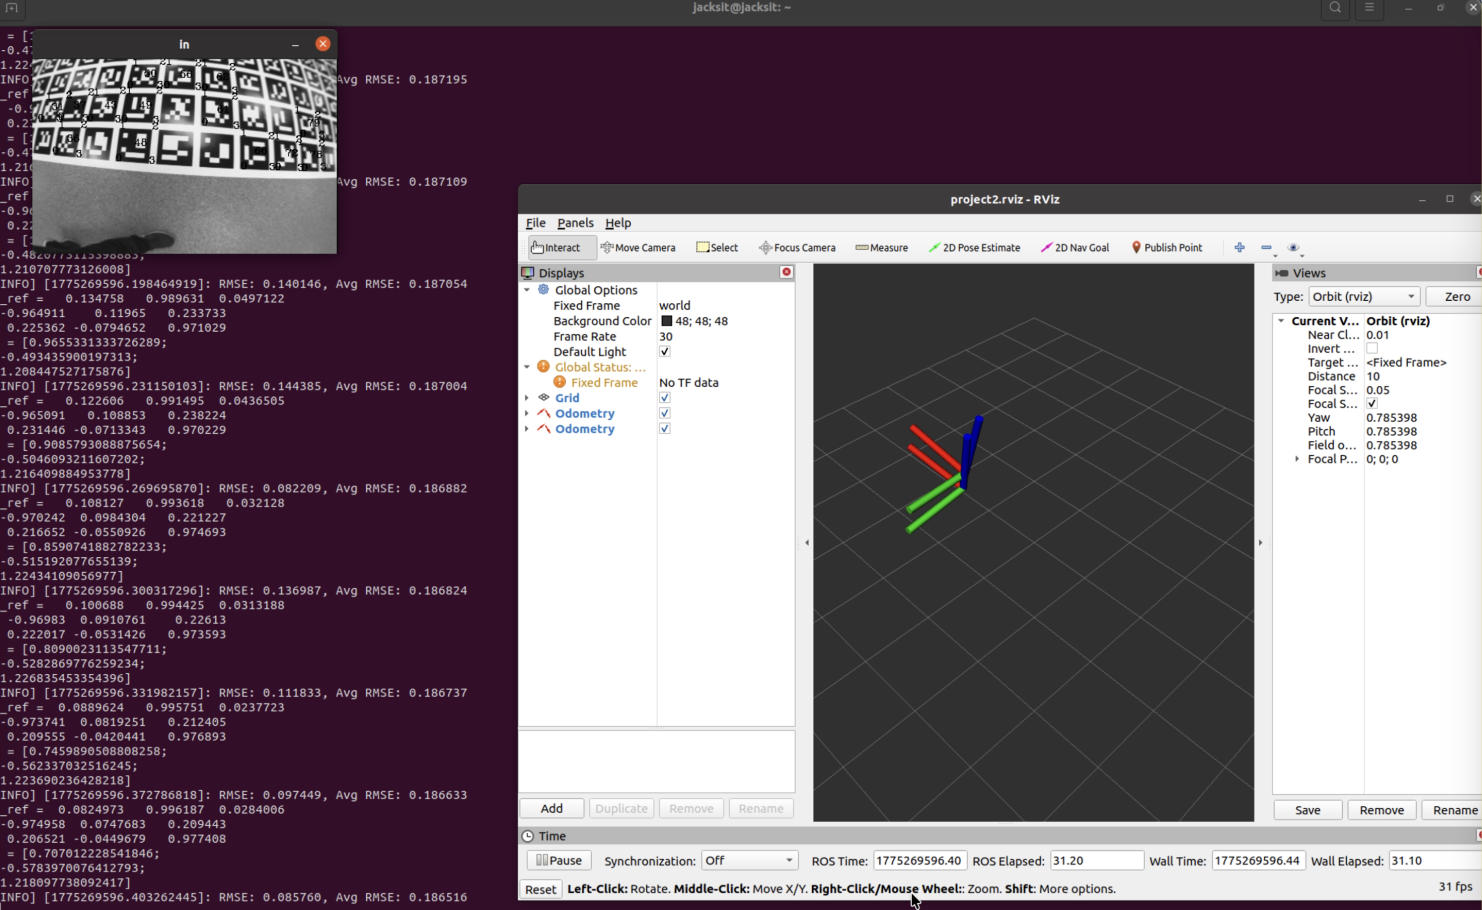
\includegraphics[width=0.45\textwidth]{assets/DLT.png}
    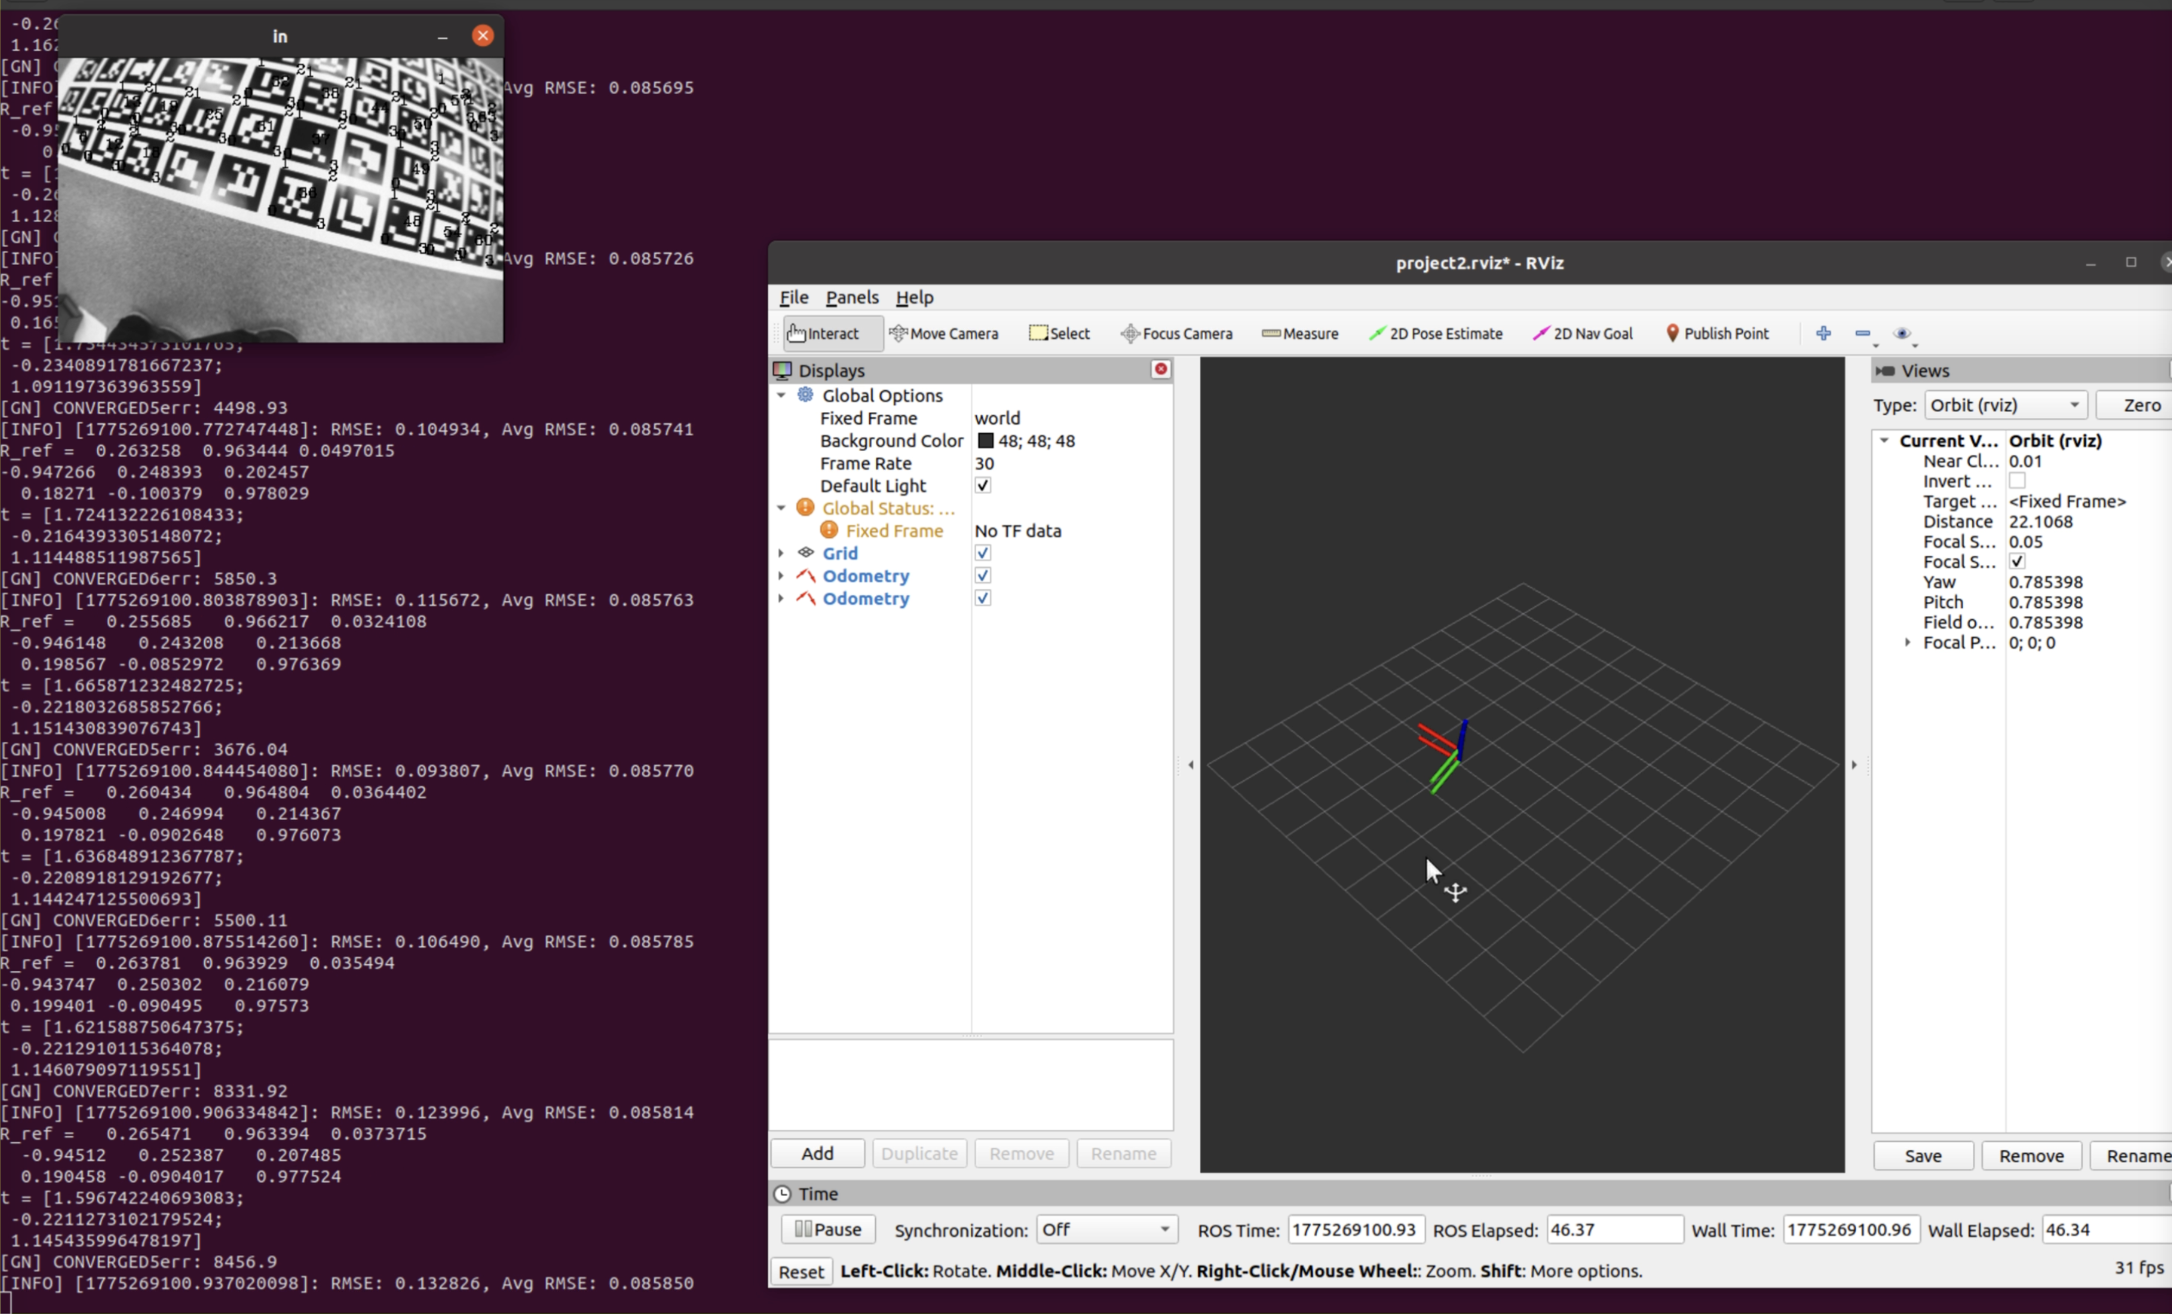
\includegraphics[width=0.45\textwidth]{assets/GN_normal.png}
    \caption{Left: DLT initialization result. Right: Refined pose after Gauss-Newton optimization.}
    \label{fig:rviz_pose}
\end{figure}

\begin{figure}[h]
    \centering
    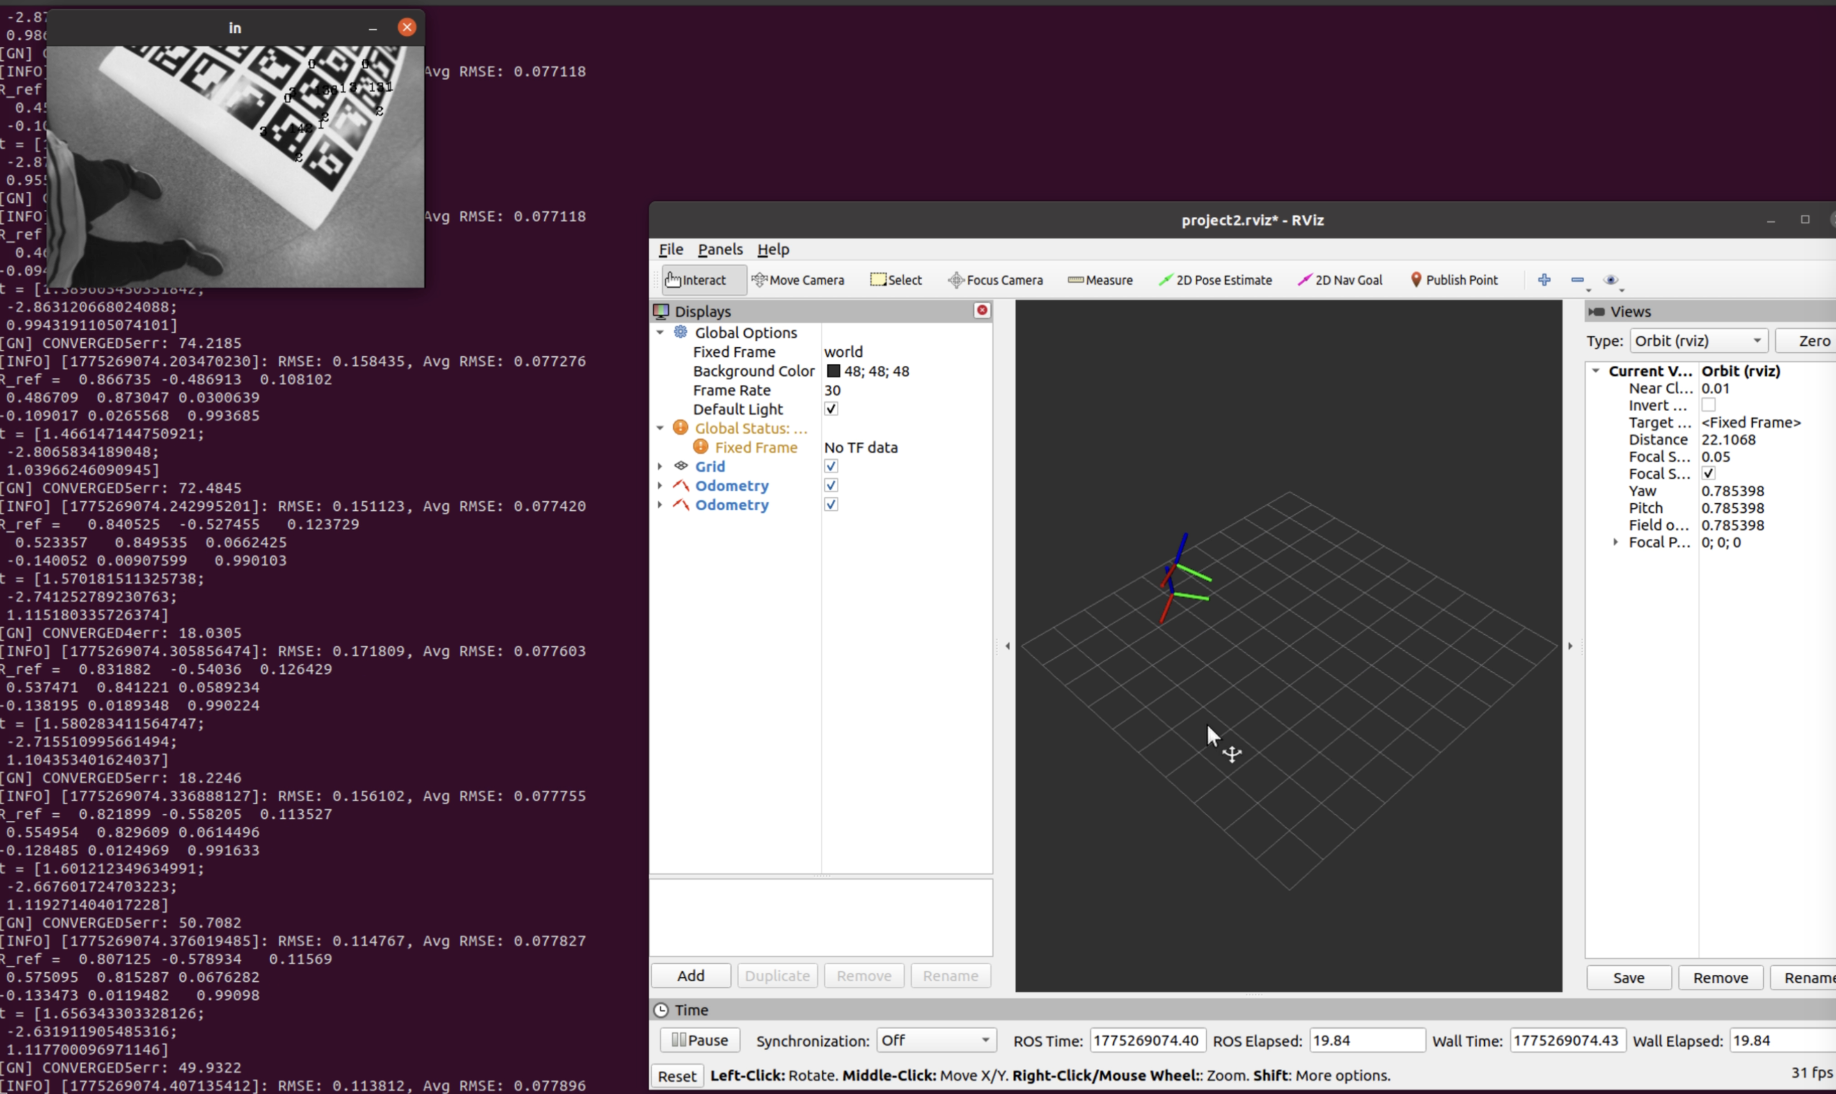
\includegraphics[width=0.45\textwidth]{assets/GN_large_error.png}
    \caption{Behavior when encountering a large error during tracking.}
    \label{fig:gn_large_error}
\end{figure}

\subsection{Statistics}
The tracking demonstrated high accuracy. Across the recorded sequence, the average Root Mean Square Error (RMSE) for the initial Direct Linear Transformation (DLT) estimation was \textbf{0.237696} pixels. After applying the Gauss-Newton nonlinear refinement, the average RMSE significantly improved to \textbf{0.092853} pixels.

\section{Analysis}
\paragraph{Accuracy:} The DLT method provided a good initial guess, but the Gauss-Newton nonlinear refinement significantly improved the accuracy by minimizing the exact geometric reprojection error. 
\paragraph{Failure Cases:} The pose estimation can become unstable when too few points are visible.

\section{References}
\begin{enumerate}
    \item ELEC 5660 Course Materials and Slides.
    \item Gao Xiang, "Visual SLAM 14 Lectures": \url{https://github.com/lishuwei0424/Self_Reference_Book_for_VSALM/blob/master/13.\%E9\%AB\%98\%E7\%BF\%94\%20\%E8\%A7\%86\%E8\%A7\%89SLAM\%E5\%8D\%81\%E5\%9B\%9B\%E8\%AE\%B2-\%E5\%AE\%8C\%E6\%95\%B414\%E8\%AE\%B2\%E7\%89\%88.pdf}
\end{enumerate}

\end{document}